\section{Type Slicing in Hazel by Example}
\label{sec:slicing-by-example}

This section previews the slicing apparatus formally introduced in later sections through three worked examples.

\Cref{fig:parse-digit-slices} demonstrates a small example of a function parsing characters to single digits. In \textbf{(a)} the function is queried for its \textit{synthesised} type, \synsrc{\texttt{Char \textrightarrow\ Option Digit}}, which is explained by just taking a single branch from the function, and the corresponding part of the \synsrc{\texttt{Digit}} type.

Secondly, \textbf{(b)} asks why the argument is \textit{required} to be a \anasrc{\texttt{Char}}, explained by an \textit{analysis} slice retaining just the function application and the \anasrc{\texttt{Char}} annotation on the function.

The formal mathematics of these two concepts is introduced in \cref{sec:synthesis,sec:analysis}, developed over a core calculus specified in \cref{sec:core-calculus} which includes sum types, products, and explicit polymorphism.

\begin{figure}[H]
\centering

\providecommand{\fold}{\gap}
% Sources of the queried type: synthesis (red) and analysis (blue).
\providecommand{\synsrc}[1]{\textcolor{BrickRed!60!gray}{#1}}
\providecommand{\anasrc}[1]{\textcolor{NavyBlue!60!gray}{#1}}
\providecommand{\synsrcS}[1]{\textcolor{red!85!black}{\textbf{\boldmath\addfontfeature{FakeBold=4.5}#1}}}
\providecommand{\anasrcS}[1]{\textcolor{blue!85!black}{\textbf{\boldmath\addfontfeature{FakeBold=4.5}#1}}}
% Purely structural skeleton: single middle shade of green.
\providecommand{\strN}[1]{\textcolor{OliveGreen!65!black}{#1}}
\providecommand{\strM}[1]{\textcolor{black!85}{#1}}
\providecommand{\strF}[1]{\textcolor{black!85}{#1}}
% Selected (focused) sub-term: soft yellow highlight
\providecommand{\focusbox}[1]{%
  \tikz[baseline=(N.base)]{%
    \node[draw=black!30, line width=0.3pt, rounded corners=2pt,
          inner sep=2pt, fill=black!10, anchor=base, align=left] (N)
         {\strut\ttfamily\bfseries #1};%
  }%
}
\providecommand{\offslice}[1]{\textcolor{black!42}{#1}}

\tikzset{
  codebox/.style={
    draw=black!55, line width=0.5pt, dotted,
    rounded corners=2.5pt, inner sep=5pt,
    align=left, anchor=north,
    font=\ttfamily\scriptsize,
  },
  querybox/.style={
    draw=black!55, line width=0.5pt, dotted,
    rounded corners=2.5pt, inner sep=5pt,
    font=\scriptsize, align=center,
    fill=black!2,
  },
  artyarrow/.style={
    -{Stealth[length=2.8mm, width=2.2mm]},
    line width=0.7pt, color=black!55,
    decorate, decoration={
      snake, amplitude=0.6mm, segment length=2.7mm,
      pre length=2mm, post length=2.5mm,
    },
  },
  arrowlbl/.style={
    font=\itshape\scriptsize, color=black!60,
    fill=white, inner sep=1.5pt,
  },
}

\begin{subfigure}[t]{0.48\textwidth}
\centering
{\textsc{\large\bfseries Synthesis slice}}\par
\smallskip

\begin{tikzpicture}
\node[codebox] (orig) at (0,0.0) {%
\strN{type} \asmref{Option}\synsrc{(A)} \strN{=} \synsrc{Some(A)} \strM{|} \offslice{None}\\
\strN{type} \asmref{Digit} \strN{=} \synsrc{Zero} \strM{|} \offslice{One | Two | $\cdots$ | Nine}\\
\strN{let} \asmref{parse\_digit} \strN{=} \synsrcS{fun} \offslice{c} \strM{:} \synsrcS{Char} \synsrcS{-\textgreater}\\
\quad\strM{case} \offslice{c} \strM{of}\\
\qquad\strF{|} \offslice{'0'} \strF{=\textgreater} \synsrcS{Some Zero}\\
\qquad\offslice{| '1' =\textgreater\ Some One}\\
\qquad\offslice{$\;\;\vdots$}\\
\qquad\offslice{| '9' =\textgreater\ Some Nine}\\
\qquad\offslice{| \_\ \ =\textgreater\ None}\\
\strN{in} \focusbox{\synsrc{parse\_digit}}\strN{(}\offslice{'5'}\strN{)}%
};

\path let \p1=(orig.north west), \p2=(orig.north east) in
  node[querybox, anchor=south west, text width={\x2-\x1-10pt}]
    (queryBox) at (\p1)
    {{\bfseries\itshape\color{black!55}select }\synsrc{\texttt{parse\_digit}}\\
     {\bfseries\itshape\color{black!55}query }$\upsilon$ = \synsrc{\texttt{Char \textrightarrow\ Option Digit}}};

\node[codebox, below=14mm of orig] (fold) {%
\strN{type} \asmref{Option}\synsrc{(A)} \strN{=} \synsrc{Some(A)} \strM{|} \fold\\
\strN{type} \asmref{Digit} \strN{=} \synsrc{Zero} \strM{|} \fold\\
\strN{let} \asmref{parse\_digit} \strN{=} \synsrcS{fun} \fold{} \strM{:} \synsrcS{Char} \synsrcS{-\textgreater}\\
\quad\strM{case} \fold{} \strM{of}\\
\qquad\strF{|} \fold{} \strF{=\textgreater} \synsrcS{Some Zero}\\
\qquad\strF{|} \fold\\
\strN{in} \focusbox{\synsrc{parse\_digit}}\strN{(}\fold\strN{)}%
};

\draw[artyarrow] (orig.south) -- node[arrowlbl] {fold} (fold.north);

% Enforce a fixed bounding box; identical coords in both subfigures guarantee
% the code segments and captions line up horizontally.
\useasboundingbox (-3.8,1.5) rectangle (3.8,-8.0);
\end{tikzpicture}

\caption{\texttt{parse\_digit} synthesises type \synsrc{\texttt{Char → Option Digit}}.}\label{fig:syn-parse-digit}
\end{subfigure}\hfill
\begin{subfigure}[t]{0.48\textwidth}
\centering
{\textsc{\large\bfseries Analysis slice}}\par
\smallskip

\begin{tikzpicture}
\node[codebox] (orig) at (0,0) {%
\offslice{type Option(A) = Some(A) | None}\\
\offslice{type Digit = Zero | One | Two | $\cdots$ | Nine}\\
\strN{let} \asmref{parse\_digit} \strN{=} \anasrc{fun} \offslice{c} \strM{:} \anasrcS{Char} \anasrc{-\textgreater}\\
\quad\offslice{case c of}\\
\qquad\offslice{| '0' =\textgreater\ Some Zero}\\
\qquad\offslice{| '1' =\textgreater\ Some One}\\
\qquad\offslice{$\;\;\vdots$}\\
\qquad\offslice{| '9' =\textgreater\ Some Nine}\\
\qquad\offslice{| \_\ \ =\textgreater\ None}\\
\strN{in} \anasrc{parse\_digit}\anasrc{(}\focusbox{'5'}\anasrc{)}%
};

\path let \p1=(orig.north west), \p2=(orig.north east) in
  node[querybox, anchor=south west, text width={\x2-\x1-10pt}]
    (queryBox) at (\p1)
    {{\bfseries\itshape\color{black!55}select }\anasrc{\texttt{'5'}}\\
     {\bfseries\itshape\color{black!55}query }$\upsilon$ = \anasrc{\texttt{Char}}};

\node[codebox, below=14mm of orig] (fold) {%
\fold\\
\fold\\
\strN{let} \asmref{parse\_digit} \strN{=} \anasrc{fun} \fold{} \strM{:} \anasrcS{Char} \anasrc{-\textgreater} \fold\\
\strN{in} \anasrc{parse\_digit}\anasrc{(}\focusbox{\fold{}}\anasrc{)}%
};

\draw[artyarrow] (orig.south) -- node[arrowlbl] {fold} (fold.north);

% Same bounding box
\useasboundingbox (-3.8,1.5) rectangle (3.8,-8.0);
\end{tikzpicture}

\caption{\texttt{'5'} analyses against type \anasrcS{\texttt{Char}}.}\label{fig:ana-parse-digit}
\end{subfigure}

\medskip
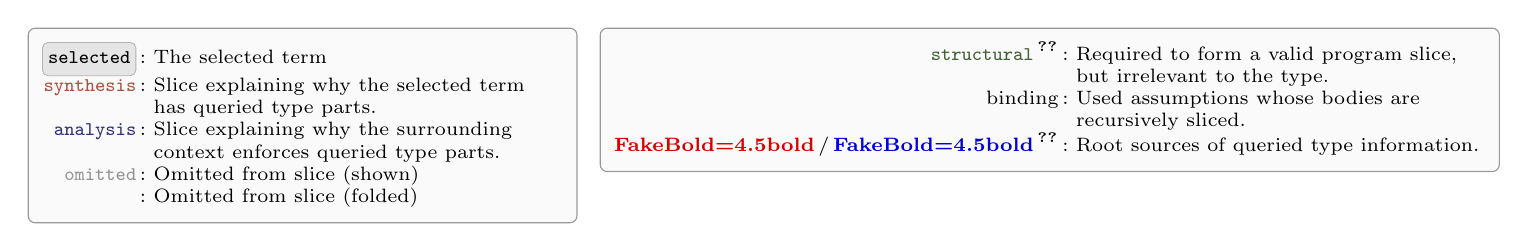
\begin{tikzpicture}
\node[draw=black!40, line width=0.4pt, rounded corners=2.5pt,
      inner sep=5pt, fill=black!2, font=\scriptsize] (lg2) {%
  \begin{tabular}{@{}r@{\,:\ }>{\raggedright\arraybackslash}p{5.2cm}@{}}
    \focusbox{selected}          & The selected term \\
    \synsrc{\texttt{synthesis}}  & Slice explaining why the selected term\newline has queried type parts. \\
    \anasrc{\texttt{analysis}}   & Slice explaining why the surrounding context enforces queried type parts. \\
    \offslice{\texttt{omitted}}  & Omitted from slice (shown) \\
    \fold                        & Omitted from slice (folded) \\
  \end{tabular}%
};
\node[draw=black!40, line width=0.4pt, rounded corners=2.5pt,
      inner sep=5pt, fill=black!2, font=\scriptsize,
      anchor=north west] (lg1) at ([xshift=8pt]lg2.north east) {%
  \begin{tabular}{@{}r@{\,:\ }>{\raggedright\arraybackslash}p{5.2cm}@{}}
    \strN{\texttt{structural}}\,\textsuperscript{\ref{fn:typesrc}} & Required to form a valid program slice,\newline but irrelevant to the type. \\
    \asmref{binding}            & Used assumptions whose bodies are recursively sliced. \\
    \synsrcS{bold}\,/\,\anasrcS{bold}\,\textsuperscript{\ref{fn:typesrc}} & Root sources of queried type information. \\
  \end{tabular}%
};
\end{tikzpicture}

\caption{Parsing a character into an \synsrc{\texttt{Option Digit}}.}
\label{fig:parse-digit-slices}
\end{figure}
\refstepcounter{footnote}\label{fn:typesrc}%
\footnotetext{The distinction between purely structural parts of a slice and bolded type sources is not formalised, but is easy to implement in practice by tagging the leaves of the derivations during slicing.}

TODO: Simplify example 2 from dissertation into a more visual Hazel example with less prose. Max one page

\Cref{sec:marking} concerns the formal theory applying type slicing to ill-typed programs with error marks, allowing for debugging of static type errors.


%%% Local Variables:
%%% mode: LaTeX
%%% TeX-master: "PolymorphicTypeSlicing"
%%% End:
